% Options for packages loaded elsewhere
\PassOptionsToPackage{unicode}{hyperref}
\PassOptionsToPackage{hyphens}{url}
%
\documentclass[
]{article}
\usepackage{amsmath,amssymb}
\usepackage{iftex}
\ifPDFTeX
  \usepackage[T1]{fontenc}
  \usepackage[utf8]{inputenc}
  \usepackage{textcomp} % provide euro and other symbols
\else % if luatex or xetex
  \usepackage{unicode-math} % this also loads fontspec
  \defaultfontfeatures{Scale=MatchLowercase}
  \defaultfontfeatures[\rmfamily]{Ligatures=TeX,Scale=1}
\fi
\usepackage{lmodern}
\ifPDFTeX\else
  % xetex/luatex font selection
\fi
% Use upquote if available, for straight quotes in verbatim environments
\IfFileExists{upquote.sty}{\usepackage{upquote}}{}
\IfFileExists{microtype.sty}{% use microtype if available
  \usepackage[]{microtype}
  \UseMicrotypeSet[protrusion]{basicmath} % disable protrusion for tt fonts
}{}
\makeatletter
\@ifundefined{KOMAClassName}{% if non-KOMA class
  \IfFileExists{parskip.sty}{%
    \usepackage{parskip}
  }{% else
    \setlength{\parindent}{0pt}
    \setlength{\parskip}{6pt plus 2pt minus 1pt}}
}{% if KOMA class
  \KOMAoptions{parskip=half}}
\makeatother
\usepackage{xcolor}
\usepackage{longtable,booktabs,array}
\usepackage{calc} % for calculating minipage widths
% Correct order of tables after \paragraph or \subparagraph
\usepackage{etoolbox}
\makeatletter
\patchcmd\longtable{\par}{\if@noskipsec\mbox{}\fi\par}{}{}
\makeatother
% Allow footnotes in longtable head/foot
\IfFileExists{footnotehyper.sty}{\usepackage{footnotehyper}}{\usepackage{footnote}}
\makesavenoteenv{longtable}
\usepackage{graphicx}
\makeatletter
\def\maxwidth{\ifdim\Gin@nat@width>\linewidth\linewidth\else\Gin@nat@width\fi}
\def\maxheight{\ifdim\Gin@nat@height>\textheight\textheight\else\Gin@nat@height\fi}
\makeatother
% Scale images if necessary, so that they will not overflow the page
% margins by default, and it is still possible to overwrite the defaults
% using explicit options in \includegraphics[width, height, ...]{}
\setkeys{Gin}{width=\maxwidth,height=\maxheight,keepaspectratio}
% Set default figure placement to htbp
\makeatletter
\def\fps@figure{htbp}
\makeatother
\setlength{\emergencystretch}{3em} % prevent overfull lines
\providecommand{\tightlist}{%
  \setlength{\itemsep}{0pt}\setlength{\parskip}{0pt}}
\setcounter{secnumdepth}{-\maxdimen} % remove section numbering
\ifLuaTeX
  \usepackage{selnolig}  % disable illegal ligatures
\fi
\IfFileExists{bookmark.sty}{\usepackage{bookmark}}{\usepackage{hyperref}}
\IfFileExists{xurl.sty}{\usepackage{xurl}}{} % add URL line breaks if available
\urlstyle{same}
\hypersetup{
  hidelinks,
  pdfcreator={LaTeX via pandoc}}

\author{}
\date{}

\begin{document}

\textbf{Imperial College London}

\textbf{Department of Earth Science and Engineering}

\textbf{MSc Environmental Data Science and Machine Learning}

\textbf{Independent Research Project Final Report}

\textbf{Predicting Individual Physiological Responses to Pollution Using
Transformer-Based Time-Series Models}

\textbf{Davide Baino}

\textbf{Email:
\href{mailto:davide.baino24@imperial.ac.uk}{\nolinkurl{davide.baino24@imperial.ac.uk}}}

\textbf{GitHub: esemsc-db24}

\textbf{Supervisors:}

\textbf{Dr. Christopher Pain}

\textbf{Dr. Boyang Chen}

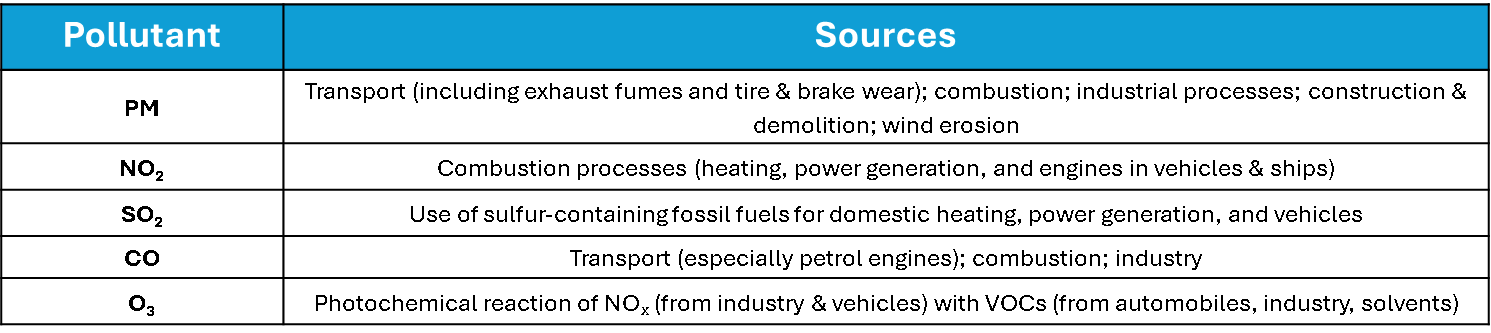
\includegraphics[width=1.77215in,height=1.8984in]{media/image1.png}

\hypertarget{table-of-contents}{%
\section{Table of Contents}\label{table-of-contents}}

\protect\hyperlink{_Toc200353825}{1. Abstract
\protect\hyperlink{_Toc200353825}{3}}

\protect\hyperlink{problem-description}{2 Problem Description
\protect\hyperlink{problem-description}{3}}

\protect\hyperlink{rationale-and-literature-review}{2.1 Rationale and
Literature Review
\protect\hyperlink{rationale-and-literature-review}{3}}

\protect\hyperlink{objectives}{2.2 Objectives
\protect\hyperlink{objectives}{4}}

\protect\hyperlink{_Toc200353829}{3 Dataset
\protect\hyperlink{_Toc200353829}{4}}

\protect\hyperlink{methodology}{4 Methodology
\protect\hyperlink{methodology}{6}}

\protect\hyperlink{_Toc200353831}{5 Timeline
\protect\hyperlink{_Toc200353831}{8}}

\protect\hypertarget{_Toc200353825}{}{}1341 UNTIL METHODOLOGY

\hypertarget{introduction}{%
\section{Introduction}\label{introduction}}

\hypertarget{abstract}{%
\section{\texorpdfstring{Abstract }{Abstract }}\label{abstract}}

Air pollution remains a major global health and environmental concern,
contributing to an estimated seven million deaths annually because of
the combined effects of outdoor and household exposure
(\href{https://www.who.int/health-topics/air-pollution\#tab=tab_2}{WHO,}
2025){[}1{]}. While pollution levels are projected to decline, the
ongoing impacts of climate change continue to pose serious risks.
Simultaneously, advancements in wearable sensor technologies allow for
the systematic collection of high-resolution physiological data over
long periods of time (Roos \& Slavich, 2023){[}2{]}.

This study aims to develop an identity map linking varying levels of air
pollution to individual physiological responses. Such a framework will
enable the prediction of health responses to pollution exposure,
facilitating early warnings and personalised health recommendations. To
achieve this, we propose a two-model approach: an initial general model
to capture general population temporal trends, and a personalised one
specialised on individual characteristics. Together, these models will
enhance the precision of forecasting and contribute to more effective,
data-driven health interventions when reacting to a polluted
environment.

\hypertarget{problem-description}{%
\section{\texorpdfstring{2. Problem Description
}{2. Problem Description }}\label{problem-description}}

\hypertarget{rationale-and-literature-review}{%
\subsection{2.1 Rationale and Literature
Review}\label{rationale-and-literature-review}}

Air pollution represents a critical challenge in the 21st century, with
significant implications for human health. For example, He et al.
{[}3{]} estimate that air pollution reduces average life expectancy by
1.8 years worldwide and up to 3 years in highly polluted regions of
China. Cardiovascular and respiratory diseases as well as lung cancer
are just some of the negative effects that the National Health System
attributes to pollution (GovUK, \emph{Health matters: Air pollution}
2018){[}4{]}.

Pollution occurs when substances from human, biological, or natural
sources enter the atmosphere at concentrations beyond typical levels,
posing short or long term risks (Bernasconi, Angelucci, \& Aliverti,
2022){[}5{]}. Pollutants are categorised as either primary, such as PM,
CO, and NO, or secondary, formed through chemical reactions like O₃ and
NO₂, often found far from their original sources. Even though this study
focused primarily on criteria pollutants such as PM₁₀ and PM₂.₅, due to
their severe health risks (Bernasconi, Angelucci, \& Aliverti,
2022){[}5{]}, other pollutants like no, no2, o3, so2, co were examined
for completeness.

Historically, air quality has been monitored using fixed-location
stations, providing aggregated environmental data at a city or regional
level. While useful for assessing general air quality trends, this
approach presents two major limitations.

Firstly, fixed locations overlooks personal exposure to pollution. These
static measurements fail to capture the highly personalised nature of
pollution exposure, which varies significantly depending on a person's
location, mobility patterns, and daily activities (Hu et al.,
2014){[}6{]}. As a result, population-level estimates often obscure the
true, specific impact of air pollution on human health (Hu et al.,
2014){[}6{]}. For instance, walking, jogging, or commuting through
high-traffic areas can expose individuals to different pollution levels
even within the same location (Hu et al., 2014){[}6{]}. The same
pollutant concentration may cause varying physiological responses across
individuals, depending on factors such as health status, age,
pre-existing respiratory conditions, and lifestyle (Hu et al.,
2014){[}6{]}.\\
Secondly, individuals inhalation rate drastically change the amount of
pollutants an individual assumes over a fixed period of time. This is
critical because including the amount of air and its relative pollution
level helps us defining the actual pollution inhalation rate of patients
rather only general pollution measures (Lu \& Fang, 2014){[}7{]}.

Recent research has improved pollution forecasting, yet gaps remain in
linking these predictions to health outcomes. For example, the Breath
study employs a transformer-based model to predict NO₂ levels in India
with high accuracy (Verma et al., 2024){[}8{]}. However, it does not
explore how these pollution fluctuations affect individual or population
health, making it not useful for policymaking or preventative
healthcare.

In contrast, Atseni et al. (2025){[}9{]} developed a machine learning
pipeline for short-term respiratory disease prediction. Their work
underscores the importance of categorise individuals before modelling
and demonstrates the effectiveness of traditional methods like Logistic
Regression, Random Forest, and XGBoost. Nevertheless, it does not
leverage modern deep learning techniques for time-series analysis, which
could better capture temporal patterns in physiological data.

\hypertarget{objectives}{%
\subsection{2.2 Objectives}\label{objectives}}

The approach proposed in this study directly addresses the challenge
outlined in the BEHRT initiative by integrating IoT-enabled wearable
devices to support proactive and personalised health interventions Li,
Y. et al. (2020){[}10{]}.

The value that this research is trying to add is not only to use
wearable devices data to quantify the physiological response to
pollution from individuals, but also to understand how much of the
pollution surrounding the individual was practically inhaled with
changing environmental conditions.

With this in mind, a transformer-based time series deep learning
variational (GAN) encoder decoder architecture has been developed. The
first objective is to leverage the transformer's strength in modelling
long-range temporal dependencies to identify population-level trends.
Thereby enabling the construction of an identity map, a variational
latent space, that relates pollution exposure to physiological
responses. The second objective is to deliver real-time, individualised
insights, alerting users to expect physiological changes when
encountering similar pollution levels in the future.

\protect\hypertarget{_Toc200353829}{}{}3. Dataset

This study combines two datasets that complement each other, allowing us
to examine how air pollution affects individual health responses.

\textbf{FIRST DATASET}

The first dataset is provided by the INHALE project (Imperial College
London, \emph{Inhale}){[}11{]} and consists of data from 59 participants
aged between 20 and 75 years, including 33 non-asthmatic and 26
asthmatic individuals. Each participant was equipped with wearable
sensors that recorded information on air pollution exposure, respiratory
health, and physical activity.

The INHALE dataset was the result of merging respiratory and pollution
patients' data at different time steps. The datasets, connected through
a common patient id identifiers , were useful to understand how
different levels of pollution, including primary and secondary would
affect individuals. Breath rate averaged over minutes or its standard
deviation were useful measures to understand patient's reactivity to
pollution.

The INHALE dataset temporal coverage was extremely limited. The data was
collected during two distinct two-week periods in summer and winter,
with non-continuous time steps. After some preprocessing , and
specifically because of transformers time series needs, data was split
into 1-hour long blocks where any shorter block was filtered out and not
considered. This was useful to give the model enough data to understand
how patterns would evolve in the long-run.

Dates and time fields also needed to be processed. Indeed, left as is,
neural networks tend to treat each timestamp as a distinct category,
focusing more on nearby ones while underestimating longer range
relationships.

To fix this, we encoded time as cyclic signals. We extracted hour, day
of week, and day of year, then mapped them onto sine and cosine
functions so that times like 23:00 and 00:00 are treated as neighbours
rather than distant values. This preserves natural cycles and helps the
model learn daily, weekly, and seasonal patterns more effectively
(Invidia Developer Forum\emph{,} 2022){[}12{]}.

\textbf{SECOND DATASET}

The second dataset, coming from OpenWeather API, provides real-time air
pollution levels, including key pollutants such as PM2.5, PM10 NO2 etc
(\emph{Current weather and forecast - openweathermap} 2025){[}13{]}.
Even though PM2.5 and PM10 were identified as the pollutants with the
greatest consequences for individuals' health, other pollutants like no,
no2 , o3 and so2 were considered for a more complete approach, as per
table below. Indeed, considering different pollutants is a good way to
summarise not only inhalation rates when commuting, but also any primary
or secondary agents inhaled when spending time indoor and outdoor
(Jonidi Jafari et al., 2021){[}14{]}.

\begin{longtable}[]{@{}
  >{\raggedright\arraybackslash}p{(\columnwidth - 2\tabcolsep) * \real{0.1346}}
  >{\raggedright\arraybackslash}p{(\columnwidth - 2\tabcolsep) * \real{0.8654}}@{}}
\toprule\noalign{}
\begin{minipage}[b]{\linewidth}\raggedright
\textbf{Pollutant}
\end{minipage} & \begin{minipage}[b]{\linewidth}\raggedright
\textbf{Sources}
\end{minipage} \\
\midrule\noalign{}
\endhead
\bottomrule\noalign{}
\endlastfoot
\textbf{PM} & Transport (including exhaust fumes and tire \& brake
wear); combustion; industrial processes; construction \& demolition;
wind erosion \\
\textbf{NO₂} & Combustion processes (heating, power generation, and
engines in vehicles \& ships) \\
\textbf{SO₂} & Use of sulfur-containing fossil fuels for domestic
heating, power generation, and vehicles \\
\textbf{CO} & Transport (especially petrol engines); combustion;
industry \\
\textbf{O₃} & Photochemical reaction of NOₓ (from industry \& vehicles)
with VOCs (from automobiles, industry, solvents) \\
\end{longtable}

\emph{Figure 1: Pollutants by source -- useful to understand impact on
patients}

The Openweather dataset is geolocated using longitude and latitude
coordinates, offering hourly pollution data at a spatial resolution of
approximately 200 metres. When matched with the individual respiratory
and pollution's data coming from the Inhale dataset, it enables a
spatially aware analysis of personal exposure to air pollution, allowing
for the integration of environmental data with individual physiological
responses. The hourly and 200-metre resolution is one of the key
limitations of this study, because it does not help us capturing highly
specific variations in pollution across different times of the day.

\textbf{MERGED DATASET}

The Inhale Dataset, coming from INHALE was therefore merged with the
OpenWeather dataset based on longitude, latitude and timestamp. This was
key, since it gives us a map of how individuals moved across London,
including different levels of indoor and outdoor pollution as well as
their physiological responses to it.

Pollution levels together with individuals' physiological responses from
patients across time and inhalation rates were the backbones of our
dataset resulting in a highly accurate and specialised model.

\hypertarget{methodology}{%
\section{4. Methodology}\label{methodology}}

1. EDA CORRELATION FEATURES

After merging the dataset and deploying data preprocessing techniques,
some exploratory data analysis was implemented so that the transformer
model could later be trained.

Outliers removal was an essential first step. Given the data collection
process and the research objectives, outliers were handled manually
rather than with standard Inter Quartile Range methods. This choice
reflects the importance of retaining real spikes, f.i. a sudden increase
in breath rate that may indicate reactions to pollution. At the same
time, implausible values were excluded, for example temperatures of 56
°C in March or pollution levels high enough to be immediately lethal.
These unrealistic records were removed from the dataset.

After removing outliers, the data was normalised. Standard normalisation
was necessary because the features had very different scales, and
without adjustment, variables with larger magnitudes would have
disproportionately influenced the model.

In addition, 12 patients were completely excluded. This is because their
breath rate average feature was missing around 30/40\% of total value,
leading to imputation as the only viable option.

After cleaning and processing the data, a correlation heatmap, as shown
in figure 2, was generated to examine relationships between features. As
expected, breath rate and physical activity features have some
correlation, greater levels of physical activity leads to more frequent
breaths and so greater breathing rate. Strong correlations also appeared
among pollution measures, consistent with the fact that polluted
environments typically contain multiple pollutants. There is no evident
correlation between physiological measures and pollution measures from
the correlation map.

A Pearson correlation heatmap, as the one below, is mainly used to
define linear relationships, while the relationship between patients'
physiological data and pollution is non-linear. Only by looking at
multi-features over different time steps we could identify any
relationship between the two.

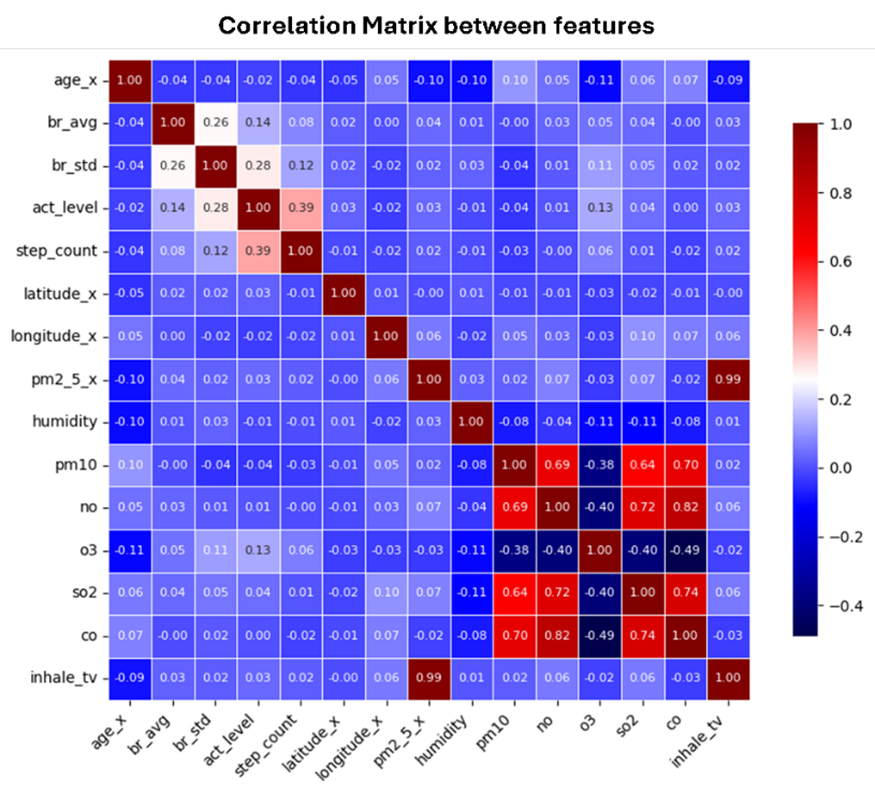
\includegraphics[width=3.976in,height=3.61037in]{media/image2.png}

\emph{Figure 2: Correlation Matrix between different features showing
strong correlation between pollution measures and between physiological
measures}

2. Data Loading -- Sliding Window Dataset

We randomly took 30 of the 44 patients for training and 13 for testing.
This is key because the model needs both healthy and asthmatic patients.
Keeping the original sequence order would have biased the results.

A custom data loader was defined and applied to both training and test
data. The first step was to determine how many windows to create using
the formula:

\textbf{Number of windows = (number of samples -- window size --
forecast steps) // step}

This shows that the number of windows depends on the dataset size,
reduced by the number of past steps and future steps, then adjusted by
the step size to optionally skip rows for memory efficiency. Each window
was then split into an input and a target. The input represents the
historical data used for training while the target is the future data
the model must predict. With this setup, the model iteratively learns by
processing each input block and predicting its corresponding target.

3. Models

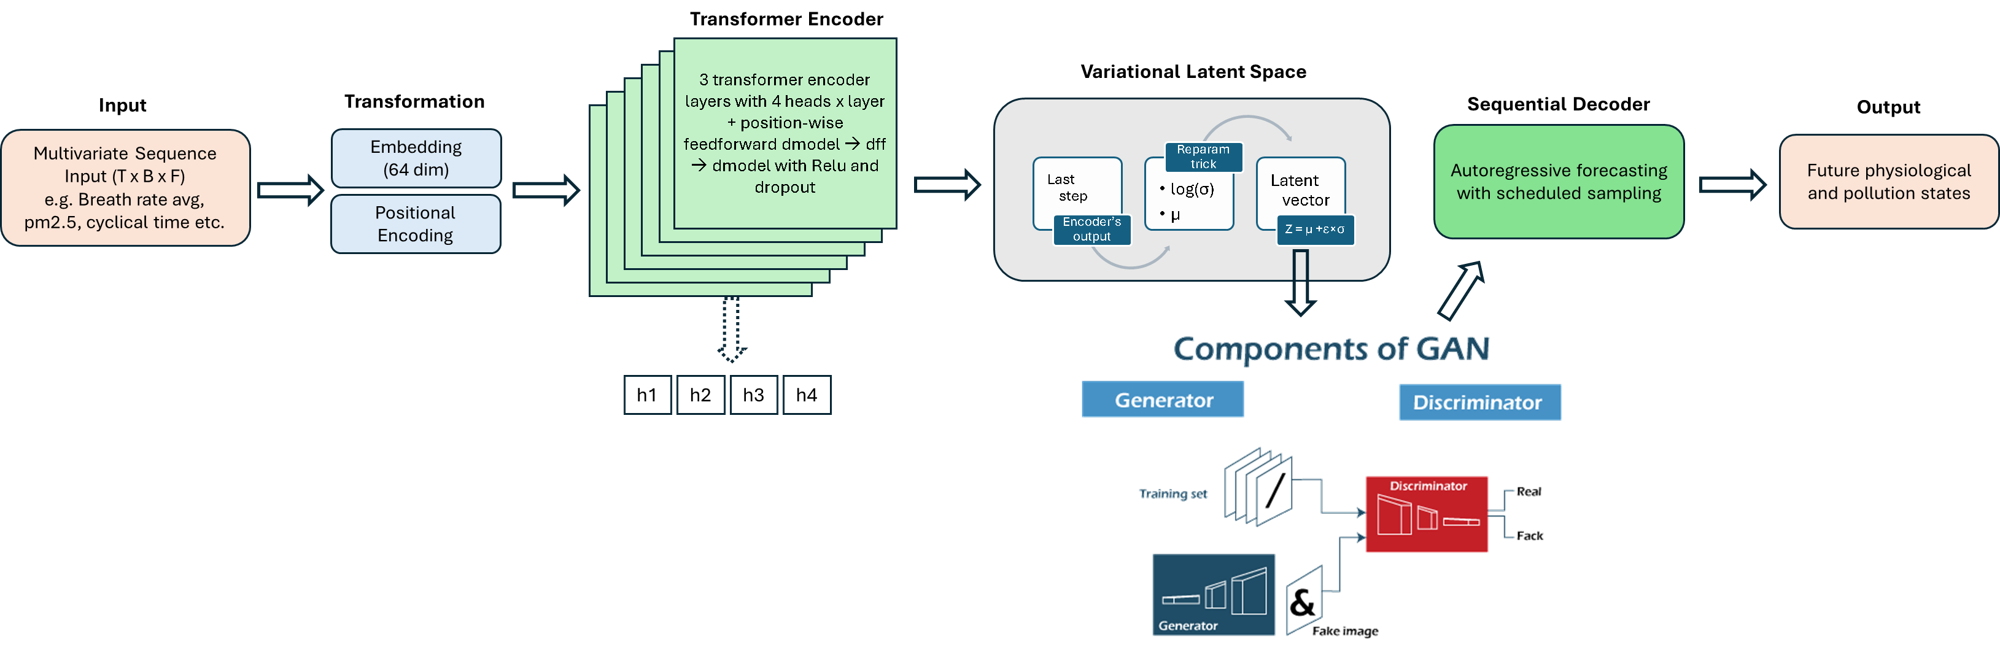
\includegraphics[width=6.83198in,height=2.03586in]{media/image3.png}

\emph{Figure 3: Transformer Vae Gan} \emph{(Thatipalli, 2023){[}15{]}
Encoder Decoder design structure}

\textbf{3.1. Customer transformer encoder}

The model takes in multivariate sequences of physiological and
environmental data, such as breathing rate, activity, and pollution
measures across different time steps. The input is structured as a 3d
tensor of sequence length, batch size and number of input features. Each
time step is embedded into a higher-dimensional vector (128 dimensions)
and with added sinusoidal positional encodings, so that temporal order
between different time steps is preserved.

Once embedded and positionally encoded, the sequence is then passed
through a stack of six transformer encoder layers.

Each encoder layer has two main parts: multi-head self-attention and a
feedforward network. Self-attention lets each time step the whole
sequence, capturing both immediate and delayed responses (Casolaro et
al., 2023){[}16{]} . This is crucial for physiological data, where
reactions to pollution may be fast or gradual. Our model uses eight
attention heads, with some attending to short-term fluctuations and
others to longer-term patterns, reflecting how individuals respond to
both recent and past exposures(Vaswani et al., 2017){[}17{]}.

After self-attention, the outputs pass through a two-layer feedforward
network with a ReLU activation in between. The first layer expands the
representation from the embedding size (d\_model) to a larger hidden
size (dim\_feedforward), giving the model more capacity to learn. ReLU
adds non-linearity, and dropout reduces overfitting by randomly dropping
activations. The second layer then projects the representation back to
the original embedding size.

\textbf{3.2 Variational Latent Space}

After the input sequence passes through the Transformer encoders, the
final hidden state is taken as a compact summary of the sequence
(dimension = d\_model). This state is projected into two vectors: a mean
(μ) and a log-variance (log(σ²)), which together define a multivariate
Gaussian distribution. Instead of mapping inputs to a single point, we
use a variational approach that samples from this distribution(Mao et
al., 2020){[}18{]}. The standard deviation is computed as:

σ = exp(0.5 × log(σ²))

To keep the sampling step differentiable, we apply the
reparameterisation trick:

s = μ + ε × σ , where ε \textasciitilde{} N(0, I)

The sampled latent vector s (typically of lower dimension f.i. 64) acts
as a bottleneck representation, keeping the key temporal information
needed for forecasting. Combining this variational latent space with the
transformer encoder allows the model to capture both temporal
dependencies and uncertainty, making it powerful for physiological
time-series prediction.

\textbf{3.3 Training}

The model is trained with an adversarial autoencoding framework designed
for time-series forecasting. Training runs in two phases.

In the first phase, a discriminator learns to distinguish between latent
vectors sampled from a standard normal distribution (s\_real) and those
generated by the encoder (s\_fake). This pushes the encoder to align its
latent space with the Gaussian prior.

In the second phase, the encoder--decoder is trained to forecast the
next block of the sequence. The loss is measured as the mean squared
error (MSE) between the predicted and actual values. Forecasting is done
autoregressively across multiple steps. To improve robustness, scheduled
sampling is applied with the model gradually shifting from using true
inputs (teacher forcing) to using its own predictions during training.

After each forward pass, a new latent vector is sampled from the
encoder's distribution, and the encoder is also trained to fool the
discriminator. This adversarial loss is weighted and added to the
reconstruction loss. A learning-rate scheduler lowers the rate when
validation loss plateaus, and early stopping prevents overfitting.

Together, these steps combine accurate forecasting with latent space
regularisation, improving both predictive performance and
generalisation.

\textbf{4. Results and discussions}

We start discussing model results by focusing on general trends from the
43 patients trained model. We begin by explaining why forecasting was
the main focus rather than reconstructing the input and we will then
analyse clustered reactions to pollution. We will delve deeper to
discover whether asthmatic individuals show stronger or weaker responses
than healthy ones. Pollution levels will then be perturbed to observe
changes in physiological measures.

After discussing general model results, we focused on generalisation by
fine-tuning the general model on data from one unseen individual.
Finally, we propose a threshold-based alert system that forecasts an
individual's physiological responses to pollution and triggers warnings
when critical thresholds are expected to exceed.

\textbf{4.1 Prediction}

Using a multimodal time series model combining pollution concentrations,
inhalation rate, and physiological signals, we predicted next-hour
physiological and pollution measures aggregated across all subjects.

As shown in figure 3, the model is able to track closely both
physiological measures such as breath average and pollution levels, with
large spikes being the hardest to capture. Two design choices are key to
this performance. The former is the ability of transformers to capture
temporal dependencies, where past inputs affect both present and future
timesteps. The latter comes from adversarial training, where generator
and discriminator are working together to make the predictions as
realistic as possible.

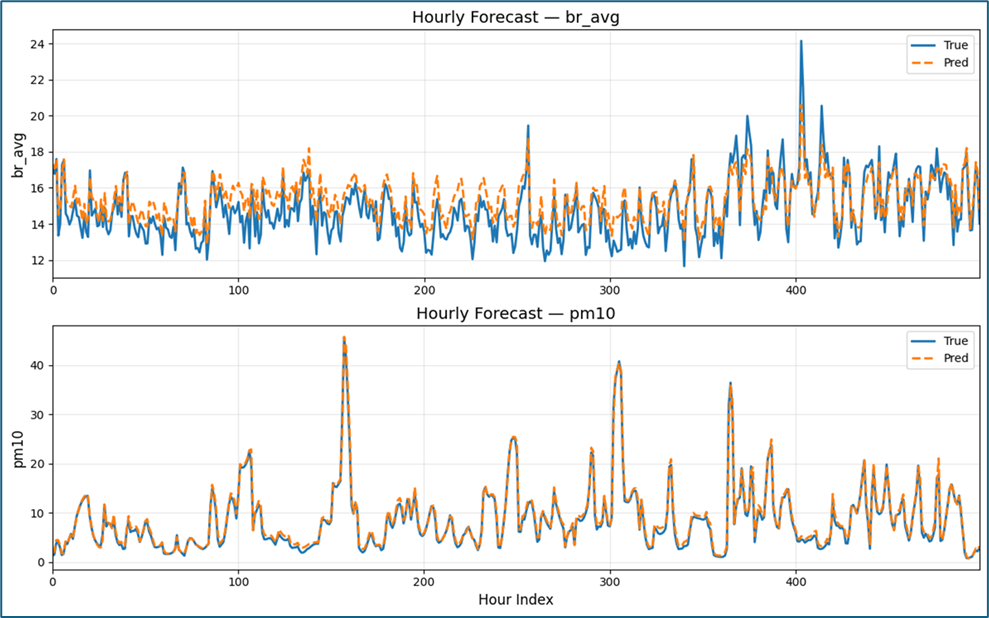
\includegraphics[width=6.56654in,height=4.09662in]{media/image4.png}

\emph{Figure 3: Prediction of breath rate average (br\_avg) and
pollution (pm10) on a hourly basis aggregated to all patients}

Also, we decided to focus on forecasting rather than reconstructing
inputs to anticipate how an individual's physiology responds to
pollution. The learned latent space captures person-specific dynamics,
making forecasts valuable to provide individuals with clear insights and
actionable support.

\begin{enumerate}
\def\labelenumi{\arabic{enumi}.}
\setcounter{enumi}{1}
\item
  \textbf{Cluster reaction to pollution (What you can't see)}
\end{enumerate}

After showing that next-step forecasting was feasible and accurate, we
analysed how patients reacted to pollution and whether subgroups had
stronger or weaker responses. For each patient, sliding windows were
passed through the model to extract latent vectors (z), which were then
averaged to produce a single embedding per individual. These embeddings
were clustered using K-Means to identify groups with similar response
patterns.

Most individuals clustered closely together, reflecting the Gaussian
distribution learned by the adversarial model, while a few formed
distinct groups, suggesting different than average physiological
response to
pollution.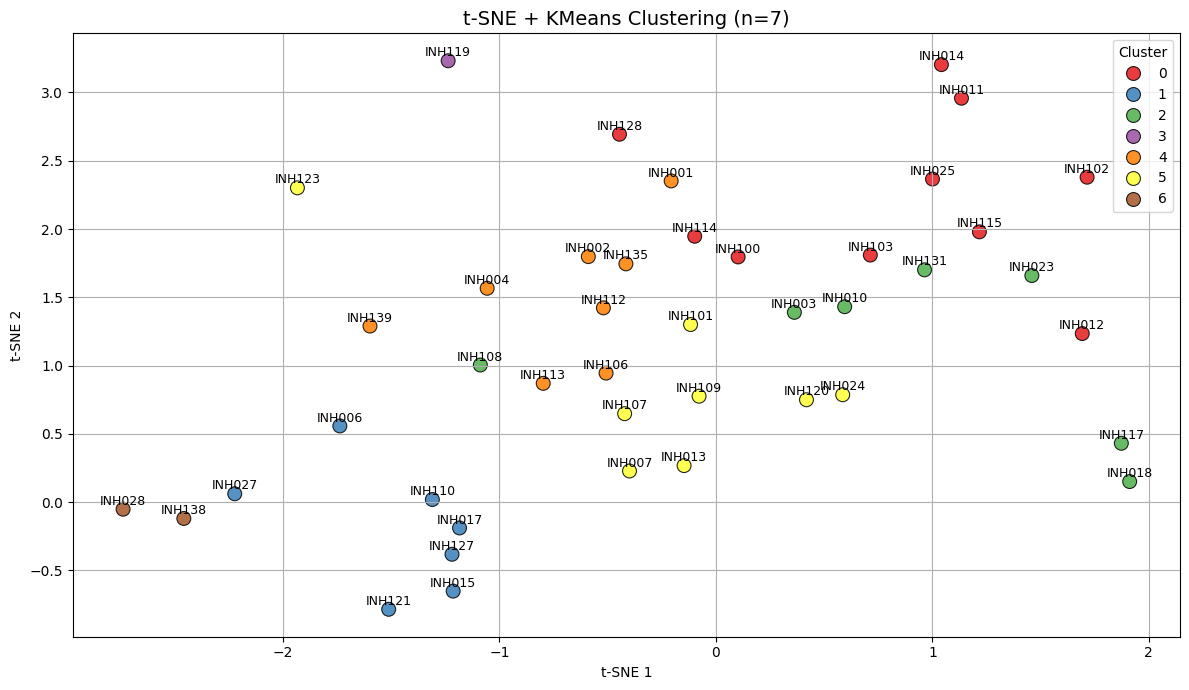
\includegraphics[width=6.26806in,height=3.63681in]{media/image5.png}

\emph{Figure 4: K-cluster for all patients in seven distinct groups
including healthy and asthmatic individuals}

For a better understanding of group-specific responses to pollution, we
examined the distributions and medians of pollution and physiological
measures across the seven clusters.

Starting with cluster 3, we can see how it was characterised by the
highest PM₂.₅ and PM₁₀ levels and shows one of the largest increases in
average breathing rate. However, it does not result in the strongest
one. This is likely because activity levels in this group are relatively
low. Cluster 4 illustrates this relationship really well: despite
slightly lower PM₂.₅/PM₁₀, higher activity levels are associated with
the strongest breathing-rate response. In contrast, Cluster 0 has modest
PM₂.₅ but elevated O₃ and SO₂ relative to other clusters, consistent
with vehicles and indoor pollution influences; individuals in this group
appear more affected by these pollutant mixtures.

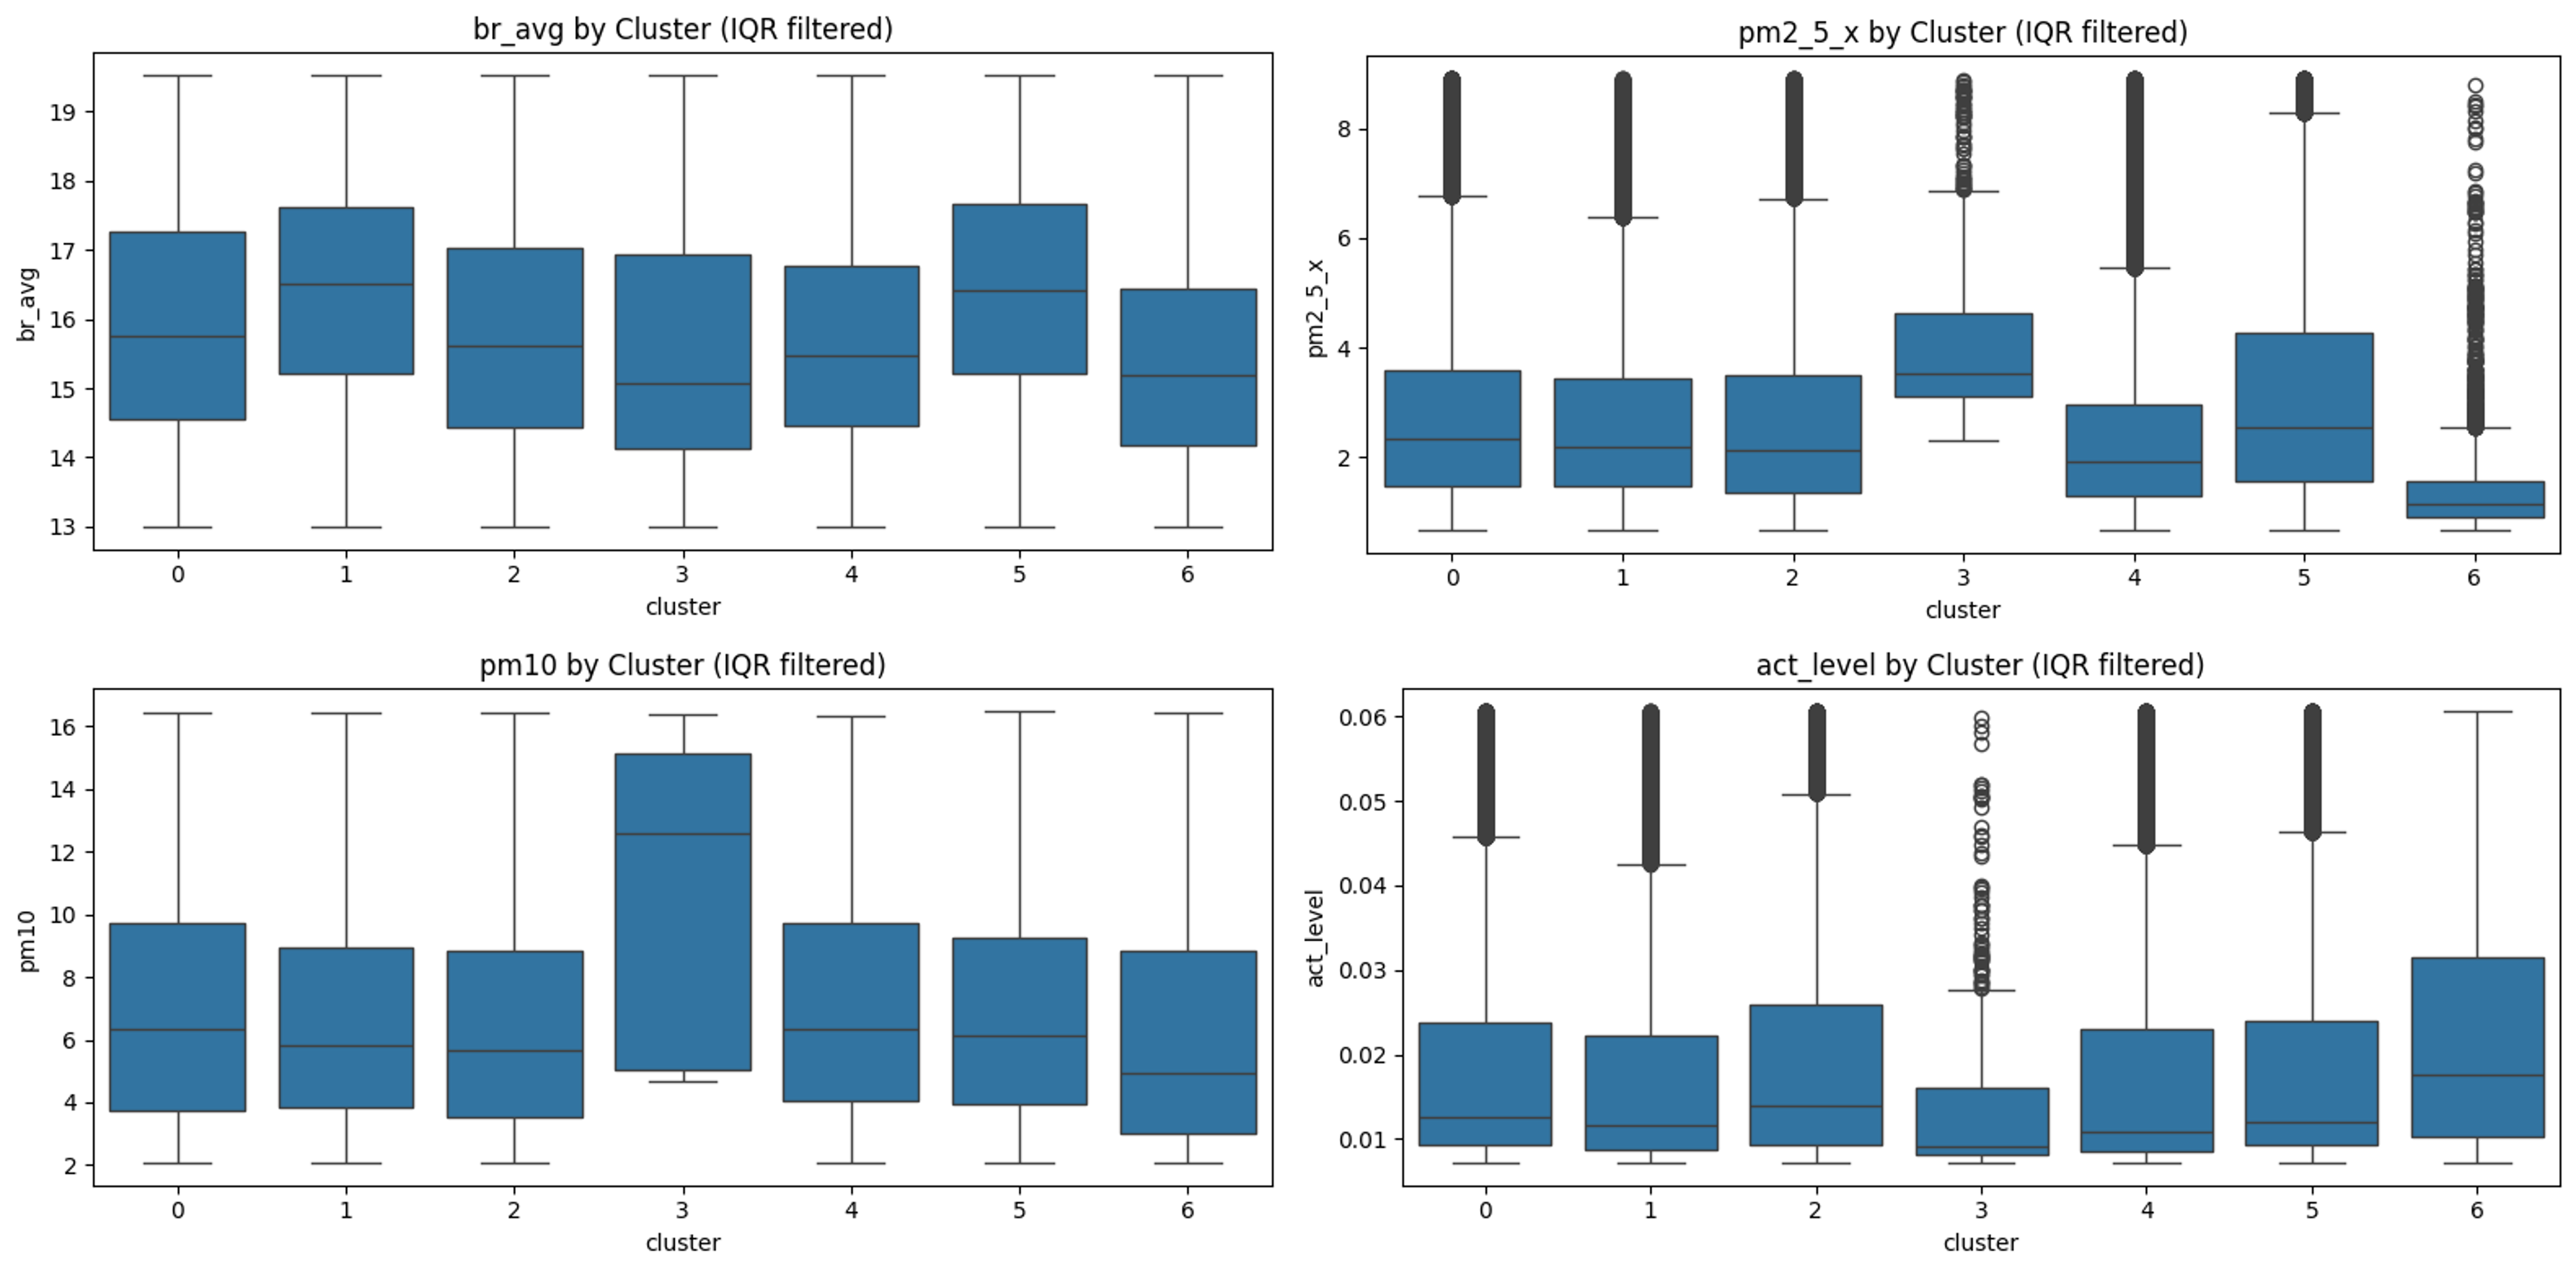
\includegraphics[width=6.4544in,height=2.92558in]{media/image6.png}

\emph{Figure 5: Distribution of breath rate average, pm2.5, activity
level and pm10 by seven clusters}

Besides clustering individuals based on their response to pollutants, we
also decided to analyse whether healthier individuals respond to
pollution any differently than asthmatic ones. We divided our dataset in
two categories, where asthmatic individuals were 19 while healthy ones
were 24. In addition, the healthy patients group have inherently more
data which involves the model being able to forecast, reconstruct and
understand healthy individuals better.

Although the literature suggests that asthmatic individuals tend to
react more strongly to pollution than healthy ones (Kim et al.,
2013){[}19{]}, our study does not show that. This was expected for a few
different reasons. Healthy individuals were exposed to higher levels of
pm2.5 than asthmatic. This, together with higher activity levels induced
a more intense level of inhalation rate across time for healthy
patients.

In practice, greater pollution exposure, higher activity levels, driven
by healthy individuals commuting more than asthmatics, resulted in a
more critical breathing-rate response among healthy participants, as
illustrated in the figure below.

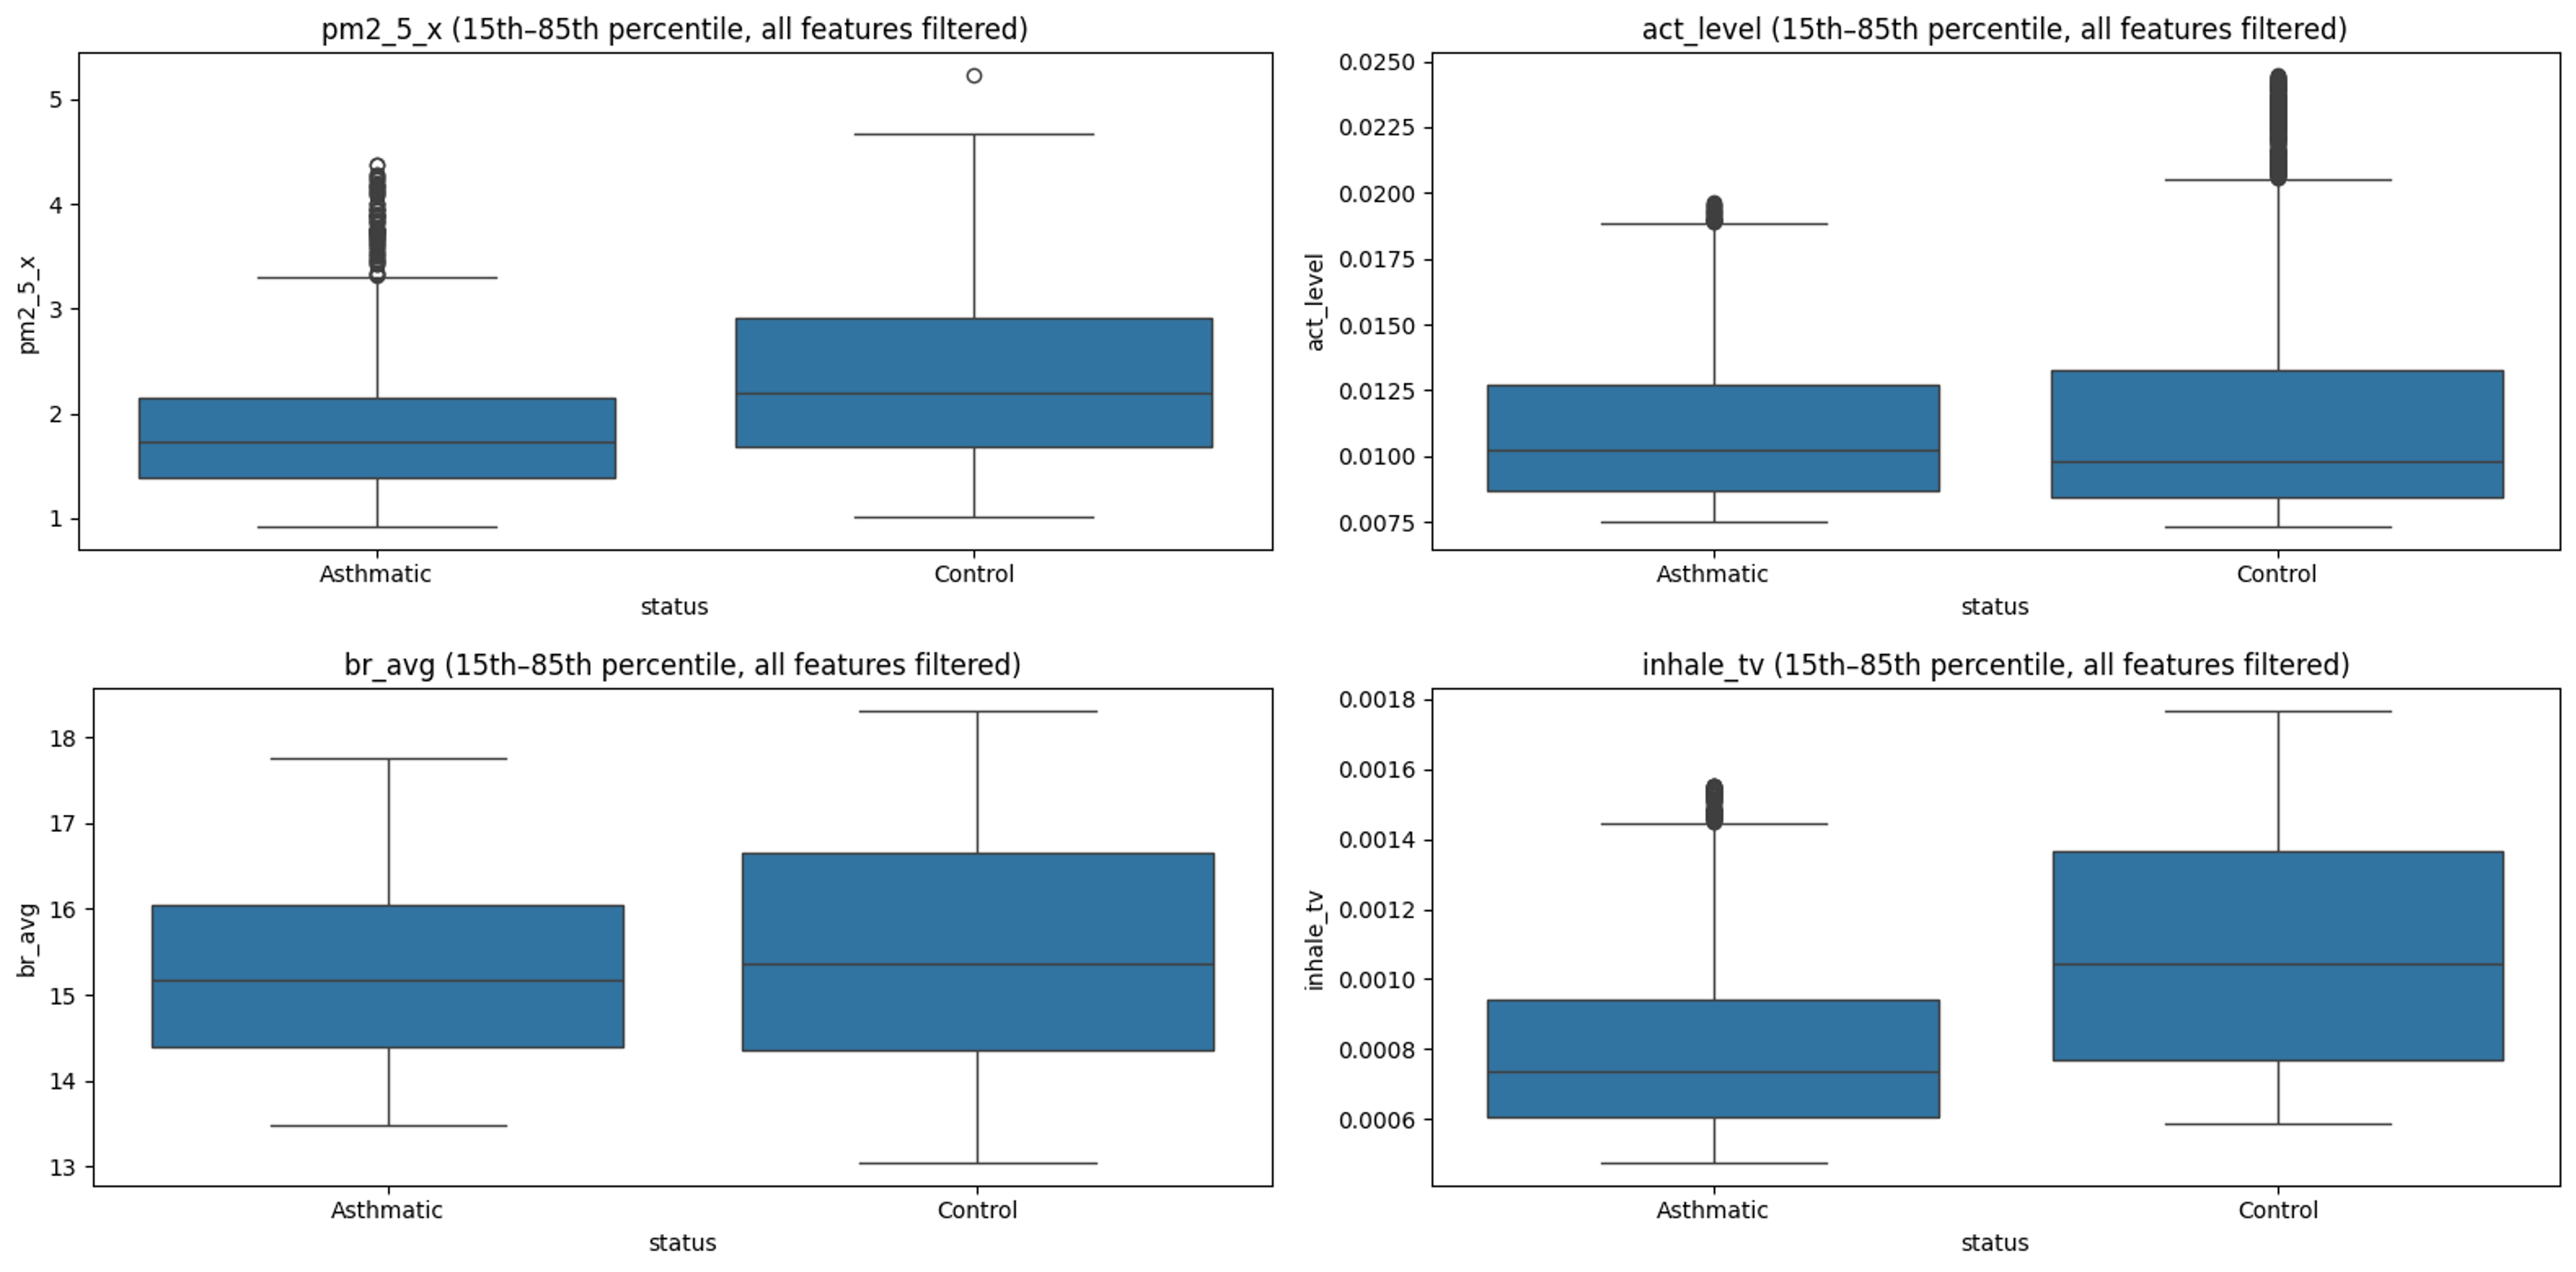
\includegraphics[width=6.36767in,height=3.14008in]{media/image7.png}

\emph{Figure 6: Distribution of pm2.5, activity, inhalation rate and
breath rate for healthy (control) vs asthmatic patients}

\begin{enumerate}
\def\labelenumi{\arabic{enumi}.}
\setcounter{enumi}{2}
\item
  \textbf{Perturbation - greater level of pollution}
\end{enumerate}

After comparing healthy and asthmatic groups, we assessed cluster-level
reactivity to pollution using a perturbation experiment. Pollution
inputs were artificially scaled (1×, 2×, 4×, 6×) while all other
variables---activity, temperature, humidity, inhalation volume, and time
encodings---remained fixed. The adjusted data was windowed, normalised
with the original scaler, and passed through the model to forecast one
step ahead. For each scenario, we examined predicted physiological
outcomes (e.g., average breathing rate) across clusters. Results were
pooled within clusters and visualised with boxplots, trimming the
10--90\% range to reduce the influence of extreme values.

From the picture below, we noticed that greater levels of pollution
leads to higher volatility within breathing rate, meaning more erratic
unstable breathing. This phenomenon is working for all the different
clusters. When looking though at breath rate average per cluster, we can
see how specific clusters, such as 1 and 3 are more reactive to
pollution while the other clusters do not react as strongly.

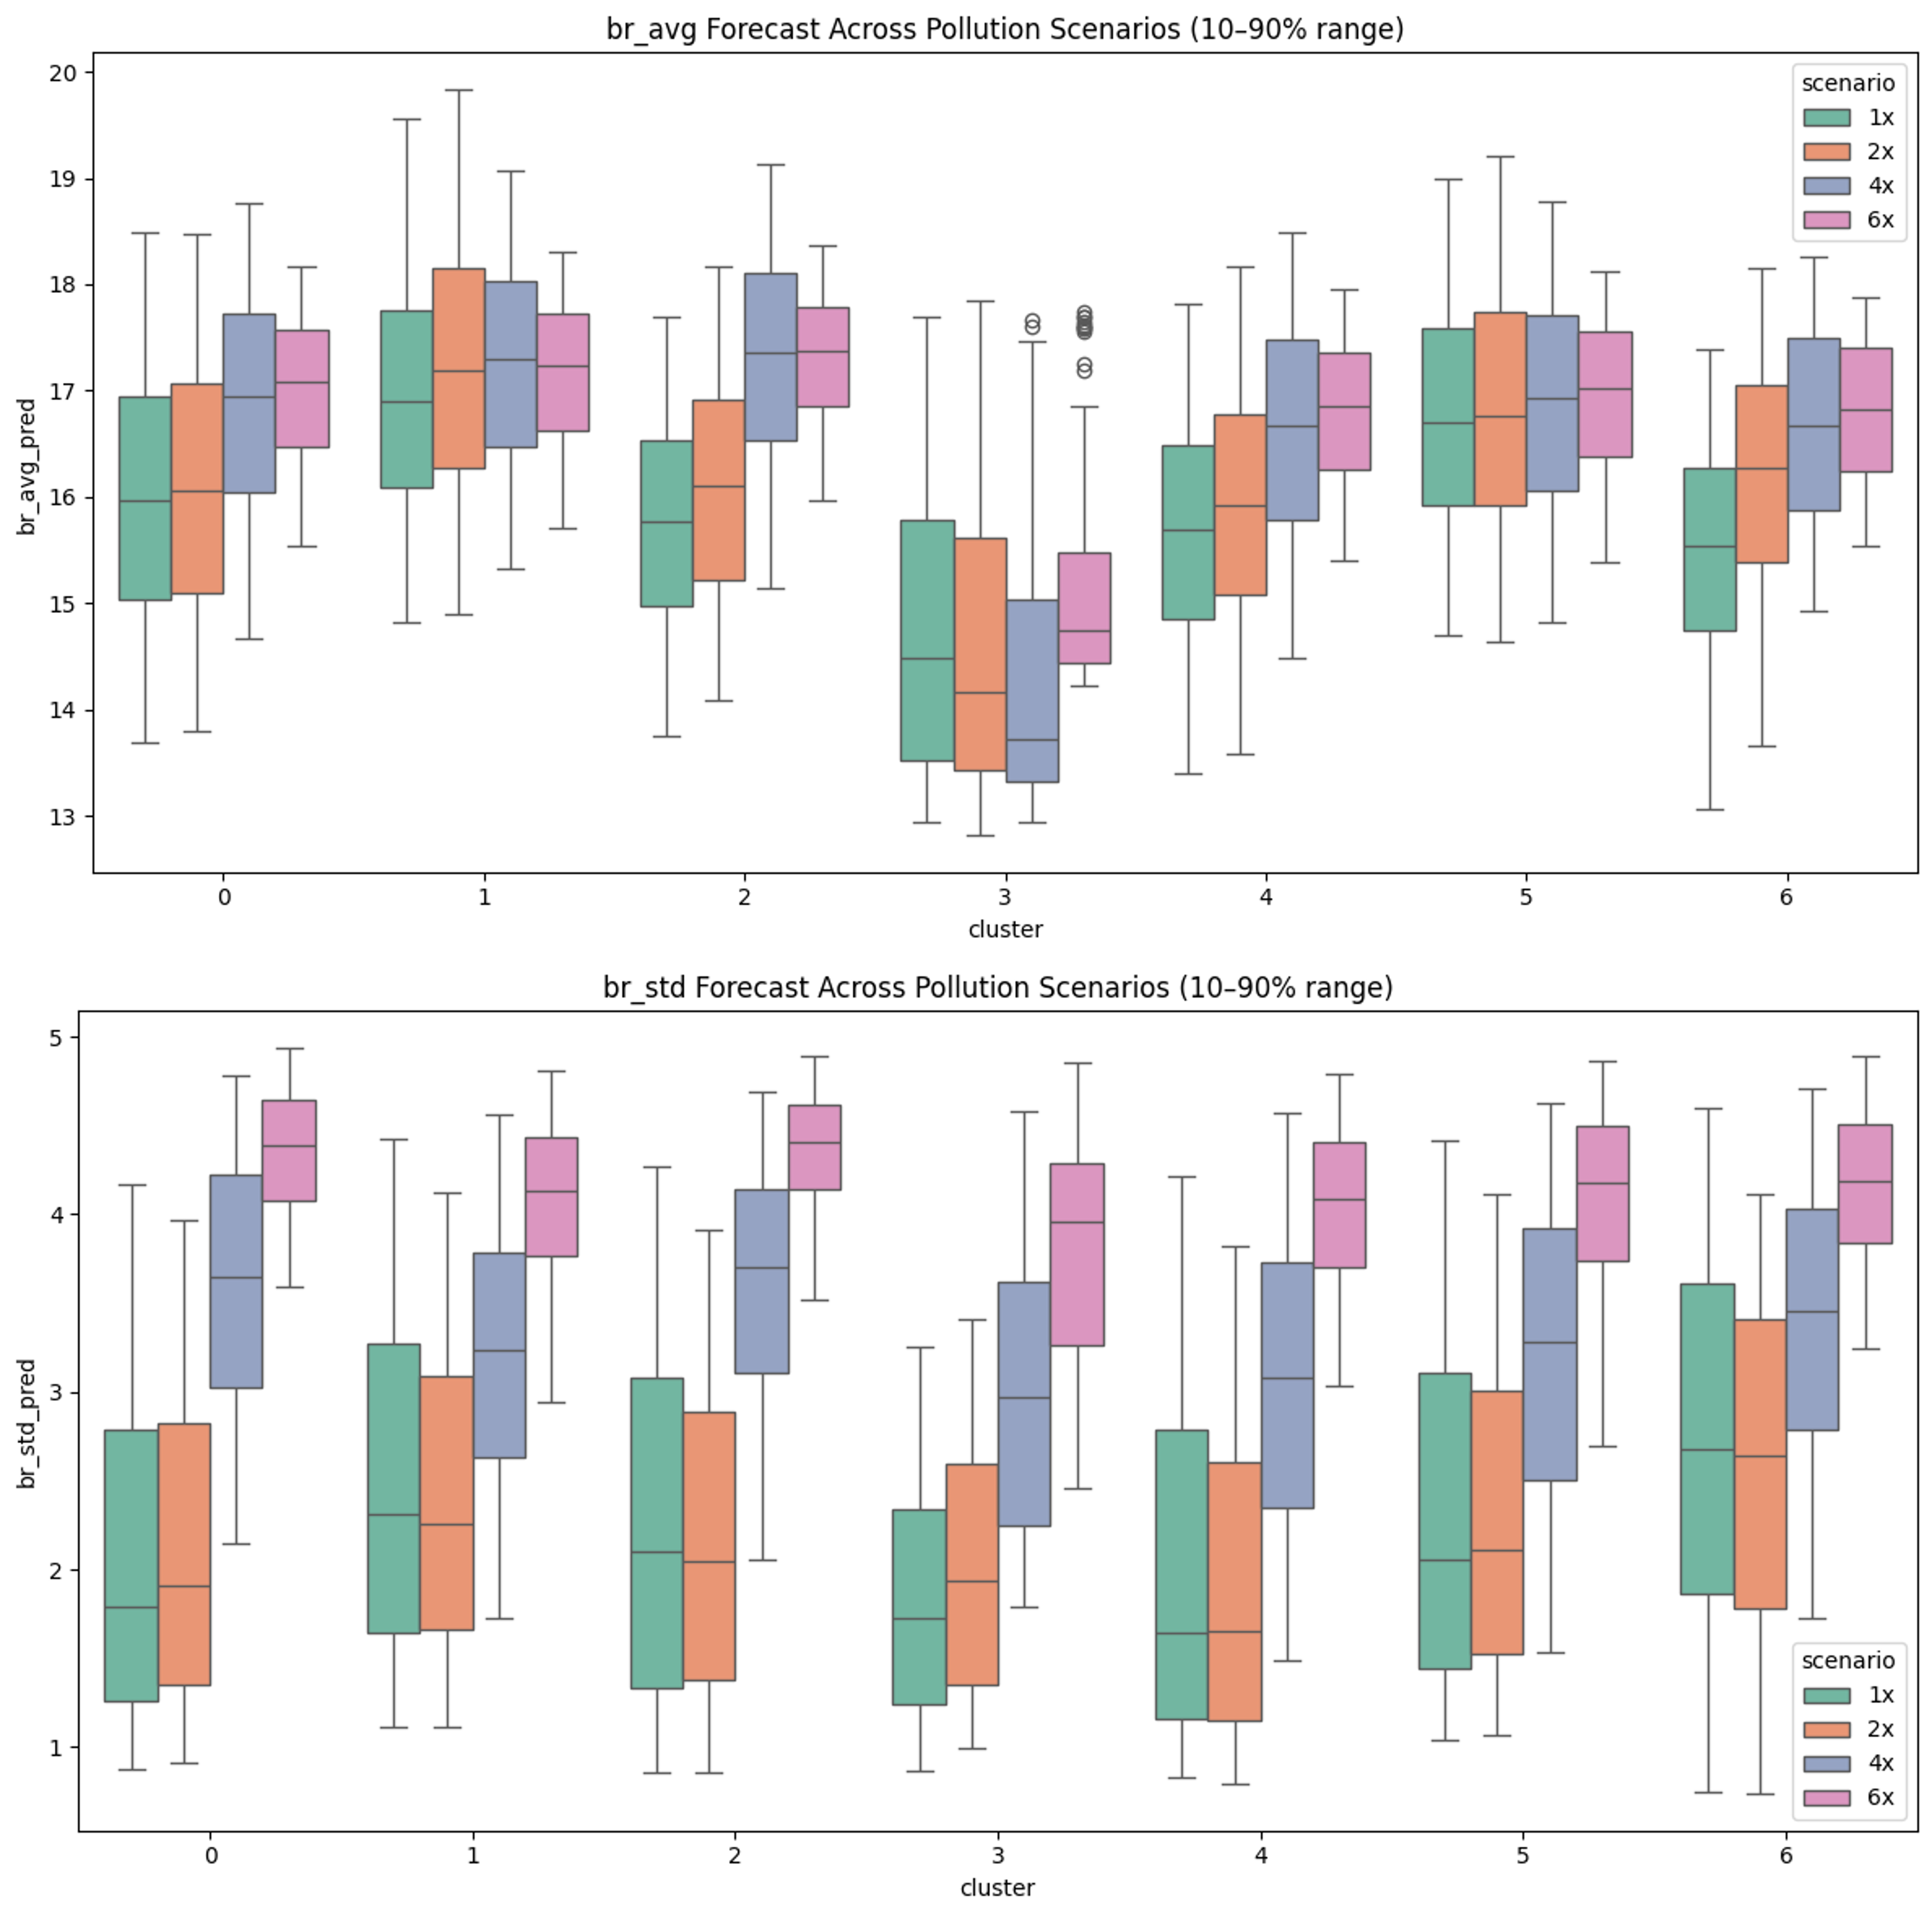
\includegraphics[width=6.17361in,height=6.16736in]{media/image8.png}

\emph{Figure 8: Perturbation of pollution measures by clusters (from 1
baseline to 6 time the baseline)}

As shown above, comparing the baseline scenario, with unchanged
pollutants inputs with the most extreme case (x6) reveals distinct
cluster-specific responses. Clusters 1, 3, and 6 show the strongest
reactivity, with breath rate rising by up to 11\%. In contrast, Clusters
0, 2, 4, and 5 display only mild changes in average breath rate but
reflect more erratic standard deviations, indicating spikier breathing
patterns.

\begin{enumerate}
\def\labelenumi{\arabic{enumi}.}
\setcounter{enumi}{3}
\item
  \textbf{Focusing on Individual only}
\end{enumerate}

After forecasting future steps for all individuals and identifying which
clusters were more or less reactive to pollution, we tested whether the
general model could generalise to unseen individuals.

As shown in figure 9, the model successfully predicted hourly
physiological responses for new patients. This shows that the model
captured general trends from the training patients while also adapting
to new features, patterns, and edge cases in unseen data. Proving its
ability to generalise to entirely new dynamics.

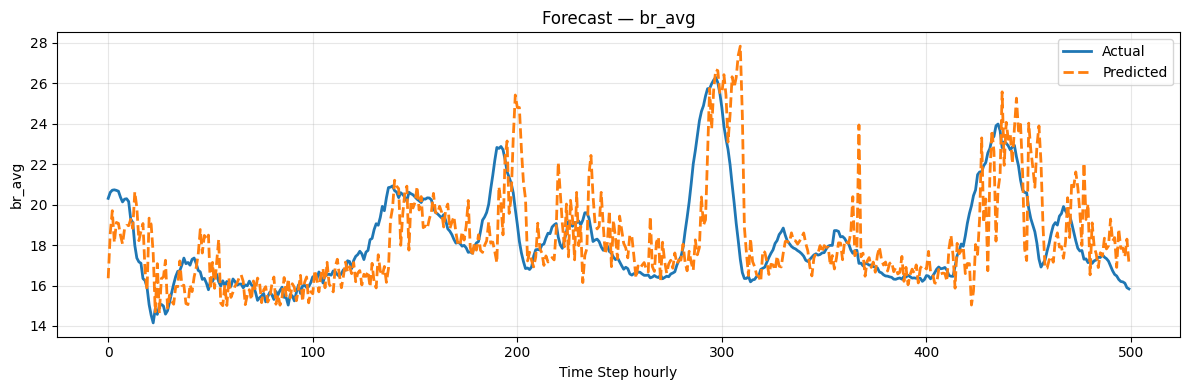
\includegraphics[width=5.59262in,height=3.72964in]{media/image9.png}

\emph{Figure 9: Forecast of unseen data hourly for both breath rate
average and standard deviation}

\textbf{4.5 Threshold -Based alert risk detection system}

The system is built to detect periods of unusual physiological change
linked to pollution exposure. It does this by first establishing a
baseline profile for each individual, then tracking deviations from that
baseline as new data arrives, and finally flagging high-risk events when
both pollution and physiological deviations are unusually high.

The baseline is created by passing all sliding windows coming from the
validation dataset through the model and extracting the first forecasted
timestep per feature. These forecasts are inverse transformed and
averaged to produce a reference vector representing the individual's
expected physiological state under normal conditions.

New forecasts are then compared to this baseline, generating a deviation
score that quantifies how far the physiology has shifted from normal
behaviour. Repeating this process creates a continuous deviation series
alongside pollution values at each timestep.

Risk was defined using percentile thresholds. Pollution values above the
75th percentile were treated as high exposure, while those below the
25th percentile were treated as low. Since these thresholds are
calculated from each individual's own data, they are customised to
different patients baseline vector, adapting automatically to different
individuals.

An alert is then triggered only when both conditions are met: pollution
exceeds its 75th percentile and the physiological deviation also exceeds
its own threshold. These events, highlighted as red dots in the final
visualisation, indicate moments when environmental stress and
physiological stress coincide. Indeed, because the alert system gets
triggered only when physiological deviation and pollution measure are
both high, false alarms are skipped. Situation where only pollution is
high but there is no reaction to it from the chosen patient, or
physiological measures deviation is abnormal but not driven by pollution
are not considered because not useful for our study. As we can see below
in figure 10, red markers highlight critical events, giving the system
the option to be an early-warning tool.

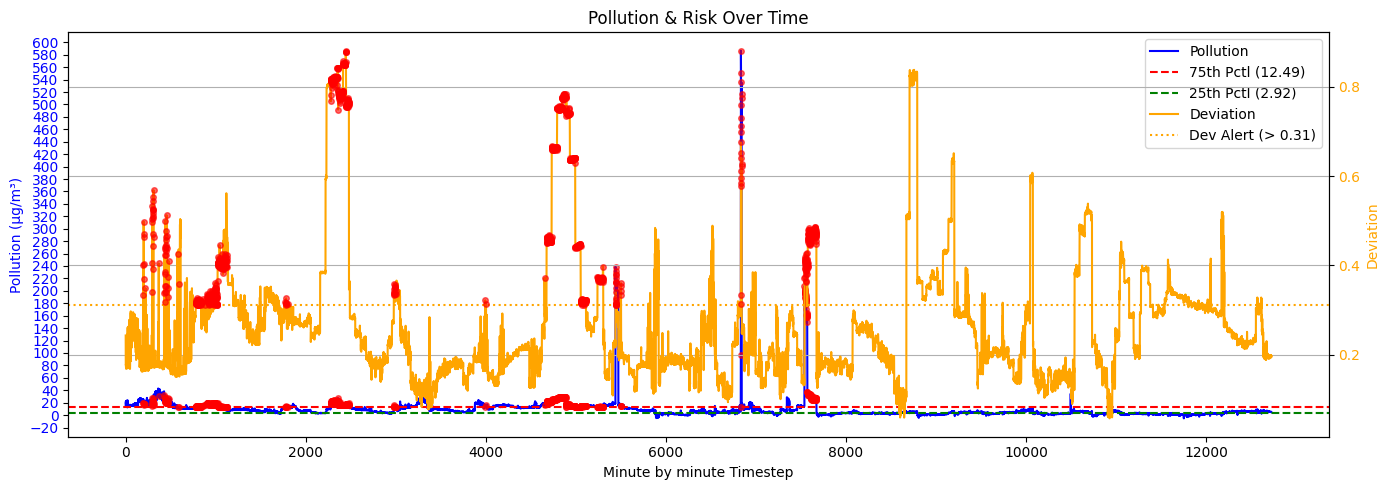
\includegraphics[width=5.64355in,height=1.99089in]{media/image10.png}

\emph{Figure 10: Hourly Threshold alerting system with pollution level
in blue, deviation from standard in yellow and red points potential
alerts.}

\textbf{5. Limitations}

Even though the overall number of patients included in the study was
representative enough, the imbalance between healthy and asthmatic makes
it skewed. Healthy individuals contributed with more data, which means
the model is better at capturing their responses compared to asthmatic
individuals.

The entire dataset was collected in London. This spatial restriction is
a key limitation because it weakens generalisability. Pollutants,
weather conditions and commuting patterns varies across different
regions, so the model won't generalise well with other cities or
countries.

The physiological measures were also limited. Breath rate and its
evolution over time is not enough to quantify the full effects of
pollution on individuals. Additional signals, such as heart rate, stress
levels would provide a more complete map of how individuals react to
pollution in the short and long-term.

The OpenWeather dataset also brings some additional limitations. Its
hourly temporal resolution, preventing minute by minute analysis, and
its 200metres spatial resolution is not able to capture
micro-environmental variations (roadside vs indoor exposure). These
limitations are especially relevant for commuting or other short-term
activities where exposure changes quickly.

Finally, the model architecture also has some limitations. The
Transformer--VAE--GAN architecture, while powerful in capturing
nonlinear temporal dependencies, operates as a black box. Its internal
representations make it difficult to attribute predictions to specific
pollutants or physiological drivers. The challenge of interpretability
reduces the model's suitability for clinical applications.

\textbf{6. CONCLUSION}

After conducting exploratory data analysis on the data, implementing
data preprocessing techniques, a clean set of data was fed to the model.
Then, a Transformer Vae Gan was trained with the aim to forecast next
time steps, including both physiological and pollution measures.

After the model has been developed and results have been comprehensively
analysed, we clearly identified that the model is precise enough to
forecast next steps both in terms of general trends but also fine-tuned
to unseen individuals. In addition, after applying a k-clustering
technique to individuals' latent space, we can see how different
clusters reactive differently to similar levels of pollutions. With some
clusters being more reactive to pollution, with spikes reaching 11\%
(when pollution is increased 6 times) while other clusters having a mild
reaction to perturbation.

In addition, a threshold alert system was developed to operationalise
the model. Indeed, being able to alert individuals on how they will
physically react when experiencing similar pollution levels could be a
great aid especially for those clusters that are very sensitive to
pollution. Another activity, or a different way to commute could be
suggested to reduce overall pollution exposure and inhalation rates.

\hypertarget{references}{%
\section{6. References}\label{references}}

\begin{enumerate}
\def\labelenumi{\arabic{enumi}.}
\item
  World Health Organisation Overview (2025) Available at:
  \url{https://www.who.int/health-topics/air-pollution\#tab=tab_1} (09
  June 2025).
\item
  Roos, L.G. and Slavich, G.M. (2023) `Wearable Technologies for health
  research: Opportunities, limitations, and practical and conceptual
  considerations', Brain, Behavior, and Immunity, 113, pp. 444--452.
  doi:10.1016/j.bbi.2023.08.008.
\item
  He, Q. and Ji, X. (James) (2021) `The labor productivity consequences
  of exposure to particulate matters: Evidence from a Chinese National
  Panel Survey', International Journal of Environmental Research and
  Public Health, 18(23), p. 12859. doi:10.3390/ijerph182312859.
\item
  Health matters: Air pollution (2018) GOV.UK. Available at:
  https://www.gov.uk/government/publications/health-matters-air-pollution/health-matters-air-pollution
  (Accessed: 14 August 2025).
\item
  Bernasconi, S., Angelucci, A. and Aliverti, A. (2022) `A scoping
  review on wearable devices for environmental monitoring and their
  application for Health and Wellness', Sensors, 22(16), p. 5994.
  doi:10.3390/s22165994.
\item
  Hu, K. et al. (2014) `Personalising pollution exposure estimates using
  wearable activity sensors', 2014 IEEE Ninth International Conference
  on Intelligent Sensors, Sensor Networks and Information Processing
  (ISSNIP), pp. 1--6. doi:10.1109/issnip.2014.6827617.
\item
  Lu, Y. and Fang, T. (2014) `Examining personal air pollution exposure,
  intake, and Health Danger Sone using time geography and 3D
  geovisualisation', ISPRS International Journal of Geo-Information,
  4(1), pp. 32--46. doi:10.3390/ijgi4010032.
\item
  Verma, A., Ranga, V. and Vishwakarma, D.K. (2024) `Breath-net: A novel
  deep learning framework for no2 prediction using bi-directional
  encoder with Transformer', Environmental Monitoring and Assessment,
  196(4). doi:10.1007/s10661-024-12455-y.
\item
  Atseni, M. et al. (2025) `A machine learning framework for short-term
  prediction of chronic obstructive pulmonary disease exacerbations
  using personal air quality monitors and lifestyle data', Scientific
  Reports, 15(1). doi:10.1038/s41598-024-85089-2.
\item
  Li, Y. et al. (2020) `Behrt: Transformer for Electronic Health
  Records', Scientific Reports, 10(1). doi:10.1038/s41598-020-62922-y.
\item
  \emph{Inhale} (2024) \emph{Imperial College London}. Available at:
  https://www.imperial.ac.uk/earth-science/research/research-projects/inhale/
  (Accessed: 14 August 2025).
\item
  Three approaches to encoding time information as features for ML
  Models (2022) NVIDIA Technical Blog. Available at:
  https://developer.nvidia.com/blog/three-approaches-to-encoding-time-information-as-features-for-ml-models/
  (Accessed: 19 August 2025).
\item
  (2025) Current weather and forecast - openweathermap. Available at:
  https://openweathermap.org/ (Accessed: 14 August 2025).
\item
  Jonidi Jafari, A., Charkhloo, E. and Pasalari, H. (2021) `Urban Air
  Pollution Control Policies and strategies: A systematic review',
  Journal of Environmental Health Science and Engineering, 19(2), pp.
  1911--1940. doi:10.1007/s40201-021-007444.
\item
  Thatipalli, A. (2023) Generative Adversarial Networks (Gans): A simple
  explanation, Medium. Available at:
  https://ai.plainenglish.io/generative-adversarial-networks-gans-a-simple-explanation-6860afda181f
  (Accessed: 19 August 2025).
\item
  Casolaro, A. \emph{et al.} (2023) `Deep learning for time series
  forecasting: Advances and open problems', \emph{Information}, 14(11),
  p. 598. doi:10.3390/info14110598.
\item
  Vaswani, A., Shaseer, N., Parmar, N., Usskoreit, J., Jones, L., Gomes,
  A.N., Kaiser, Ł. \& Polosukhin, I., 2017. Attention is all you need.
  In Advances in Neural Information Processing Systems (NIPS 2017).
\item
  Mao, X. and Li, Q. (2020) `Generative Adversarial Networks (gans)',
  Generative Adversarial Networks for Image Generation, pp. 1--7.
  doi:10.1007/978-981-33-6048-8\_1.
\item
  Kim, K.-H., Jahan, S.A. and Kabir, E. (2013) `A review on human health
  perspective of air pollution with respect to allergies and asthma',
  Environment International, 59, pp. 41--52.
  doi:10.1016/j.envint.2013.05.007.
\end{enumerate}

\end{document}
